\documentclass[11pt,a4paper]{article}
\usepackage[margin=1in]{geometry}
\usepackage{booktabs}
\usepackage{amsmath}
\usepackage{hyperref}
\usepackage{graphicx}
\usepackage{microtype}
\usepackage{parskip}
\usepackage{caption}

\title{\textbf{CSI500 Stock Selection Competition}\\[0.4em]
       \large Machine Learning (Spring 2026)}
\author{ch5085@nyu.edu}
\date{Submission 1: 2026-05-03 \quad Submission 2: 2026-05-10}

\begin{document}
\maketitle
\tableofcontents
\newpage

%% ============================================================
\section{Factors}
%% ============================================================

\subsection{Baseline Features (14)}

The competition baseline provides 14 features: multi-horizon returns
(\texttt{ret\_1d} through \texttt{ret\_60d}), realised volatility
(\texttt{vol\_5d}, \texttt{vol\_20d}), volume z-score, turnover MA,
moving-average distances (\texttt{close\_over\_ma20},
\texttt{close\_over\_ma60}), RSI-14, and cross-sectional percentile
ranks of returns and volatility. Cross-sectional ranking is applied
to all raw signals to make features robust to the heteroskedastic
return distributions across the CSI500 universe.

\subsection{Extended Technical Features (+14)}

\begin{table}[h]
\centering
\begin{tabular}{lll}
\toprule
Feature & Formula / Window & Intuition \\
\midrule
\texttt{macd}, \texttt{macd\_signal}, \texttt{macd\_hist}
  & EMA(12,26,9), price-normalised & Trend / momentum \\
\texttt{bb\_position}
  & $(close - lower)/(upper - lower)$, 20d Bollinger & Relative price position \\
\texttt{ret\_accel\_5d}
  & \texttt{ret\_5d} $-$ \texttt{ret\_5d.shift(5)} & Momentum acceleration \\
\texttt{ret\_skew\_20d}, \texttt{ret\_kurt\_20d}
  & Rolling 20d skew / kurtosis of \texttt{ret\_1d} & See below \\
\texttt{hl\_range\_ma\_20d}
  & 20d mean of $(high-low)/close$ & Intraday volatility \\
\bottomrule
\end{tabular}
\caption{Extended technical features.}
\end{table}

\textbf{Motivation for skewness and kurtosis in A-shares.}
Retail investors dominate the CSI500 and exhibit strong lottery-seeking
behaviour. Stocks with high 20-day positive skewness have recently
generated one or more large daily gains, attracting retail buying and
driving prices above fundamental value --- a pattern that typically
reverses over the following week. Kurtosis captures fat tails
and is associated with elevated short-term volatility risk; stocks with
high kurtosis tend to have wider bid-ask spreads and higher uncertainty
around future returns.

\subsection{A-Share Alpha Factors (+14)}

\begin{table}[h]
\centering
\begin{tabular}{lp{5cm}p{4.5cm}}
\toprule
Feature & Definition & Hypothesis \\
\midrule
\texttt{amihud\_20d}
  & 20d mean of $|ret_{1d}| / amount \times 10^8$
  & Illiquidity premium (Amihud 2002): illiquid stocks
    command higher expected returns \\
\texttt{max\_ret\_20d} / \texttt{min\_ret\_20d}
  & Rolling 20d max / min single-day return
  & MAX factor: lottery demand $\rightarrow$ reversal;
    MIN: oversold bounce \\
\texttt{price\_to\_52w\_high/low}
  & $close / rolling\_max(252) - 1$
  & 52-week anchoring and mean reversion \\
\texttt{turnover\_z\_60d}
  & z-score of 5d turnover vs 60d baseline
  & Abnormal activity predicts reversal \\
\texttt{overnight\_ret}
  & $open_t / close_{t-1} - 1$
  & Informed overnight order flow \\
\texttt{intraday\_ret}
  & $close_t / open_t - 1$
  & Retail-driven intraday component \\
\texttt{streak}
  & Consecutive up/down days
  & Momentum exhaustion \\
\bottomrule
\end{tabular}
\caption{A-share specific alpha factors.}
\end{table}

\subsection{Industry Neutralisation}

\textbf{Data source.}
SW Level-1 industry labels (申万一级行业) are stored in
\texttt{data/industry.csv}, which maps each stock code to one SW Level-1
sector via the column \texttt{sw1\_industry}. The file is joined to the
price panel on \texttt{stock\_code} inside \texttt{\_industry\_neutralize()}
in \texttt{features\_enhanced.py} before any cross-sectional computation.
Stocks not present in the file are assigned to a catch-all
\texttt{"Unknown"} group.

\textbf{Procedure.}
When \texttt{industry\_neutral=True}, \texttt{build\_features()} subtracts
the daily cross-sectional mean of each SW Level-1 group from (a) the
5-day forward return target and (b) all return-based features, before
computing percentile ranks. This forces the model to learn stocks that
outperform their own sector peers rather than simply loading on
sector-rotation signals.

\textbf{Effect.} Rank IC on the test set improved from $-0.009$ (no
neutralisation) to $+0.026$ (with neutralisation).

\subsection{Feature Importance}

Table~\ref{tab:fimp} shows the top-20 features by LightGBM split
importance, trained on the full training set.

\begin{table}[h]
\centering
\begin{tabular}{clr}
\toprule
Rank & Feature & Importance \\
\midrule
1  & \texttt{amihud\_20d}          & 54 \\
2  & \texttt{hl\_range\_ma\_20d}   & 43 \\
3  & \texttt{ma20\_over\_ma60}     & 43 \\
4  & \texttt{turnover\_ma\_20d}    & 43 \\
5  & \texttt{vol\_60d}             & 42 \\
6  & \texttt{amihud\_20d\_rank}    & 36 \\
7  & \texttt{ret\_20d}             & 33 \\
8  & \texttt{macd\_signal}         & 32 \\
9  & \texttt{ret\_kurt\_20d}       & 30 \\
10 & \texttt{ret\_skew\_20d}       & 29 \\
11 & \texttt{min\_ret\_20d\_rank}  & 27 \\
12 & \texttt{overnight\_ratio\_20d}& 26 \\
13 & \texttt{turnover\_z\_60d\_rank}& 26 \\
14 & \texttt{min\_ret\_20d}        & 25 \\
15 & \texttt{price\_to\_52w\_low}  & 25 \\
16 & \texttt{close\_over\_ma5}     & 24 \\
17 & \texttt{macd}                 & 23 \\
18 & \texttt{macd\_hist}           & 23 \\
19 & \texttt{vol\_20d}             & 21 \\
20 & \texttt{price\_to\_52w\_high\_rank} & 20 \\
\bottomrule
\end{tabular}
\caption{Top-20 features by LightGBM split importance.}
\label{tab:fimp}
\end{table}

Signal is reasonably distributed: \texttt{amihud\_20d} leads (liquidity
premium dominates in A-shares), followed by volatility-range measures and
trend indicators. No single feature accounts for more than 10\% of total
importance, indicating the model does not rely on any one signal.

%% ============================================================
\section{Models and Portfolio Construction}
%% ============================================================

\subsection{Train / Validation / Test Split}

\begin{table}[h]
\centering
\begin{tabular}{llll}
\toprule
Split & Date Range & Approx.\ Rows & Purpose \\
\midrule
Train     & 2022-01-01 $\to$ 2024-09-30 & $\sim$196{,}000 & Model fitting \\
(embargo) & 2024-10-01 $\to$ 2024-10-31 & ---             & $\geq 5$ trading-day buffer \\
Validation& 2024-11-01 $\to$ 2025-05-31 & $\sim$69{,}000  & Hyperparameter selection only \\
(embargo) & 2025-06-01 $\to$ 2025-06-30 & ---             & $\geq 5$ trading-day buffer \\
Test      & 2025-07-01 $\to$ 2026-05-08 & $\sim$100{,}000 & Final held-out evaluation \\
\bottomrule
\end{tabular}
\caption{Train / validation / test split with embargo gaps.}
\end{table}

\textbf{Forward-return target.} The prediction target is the 5-trading-day
forward return: $r_{t,t+5} = close_{t+5}/close_t - 1$, computed via
\texttt{.shift(-5)} within each stock's own time series ($h = 5$).
Training frames exclude the last $h$ rows of each window so that no future
price enters any training label.

\textbf{Look-ahead prevention.} All rolling features use only past
observations. An embargo gap of at least 5 trading days separates the end
of each training window from the start of the validation/test window,
ensuring no label leakage across splits.

\textbf{Hyperparameter selection procedure.}
\begin{itemize}
  \item \emph{Training window start (2022-01-01):} Scanned candidate years
        \{2020, 2021, 2022, 2023\} and selected the year with the highest
        mean rank IC on the \emph{validation} set. Test data was never
        consulted.
  \item \emph{Rolling lookback (500 trading days):} Compared 250d, 500d, and
        full history via validation IC. 500d was selected.
  \item \emph{LightGBM architecture} (\texttt{max\_depth=6},
        \texttt{num\_leaves=63}, \texttt{min\_child\_samples=20},
        \texttt{subsample=0.8}, \texttt{colsample\_bytree=0.7}): set based
        on standard LightGBM best practices for medium-sized tabular data,
        then lightly verified on validation IC. No exhaustive grid search
        was performed.
  \item \emph{n\_estimators:} During the walk-forward backtest, early
        stopping (patience 50) on the validation tail determined the
        typical best iteration range. For the live submissions, the
        validation tail is only $\sim$10 days --- too short for reliable
        early stopping (it triggers at round 1--2). A fixed 180 rounds,
        consistent with the walk-forward median best iteration, was used
        instead.
\end{itemize}

\subsection{Models Evaluated}

\textbf{XGBoost baseline (14 features).}
The competition-provided baseline with \texttt{early\_stopping\_rounds=30}
on the validation split.
\begin{verbatim}
n_estimators=400, max_depth=5, learning_rate=0.05
subsample=0.8, colsample_bytree=0.8, min_child_weight=10
reg_lambda=1.0, early_stopping_rounds=30
\end{verbatim}

\textbf{Final model: LightGBM with walk-forward retraining (52 features).}
\begin{verbatim}
n_estimators=180 (fixed, for submission)
learning_rate=0.03, max_depth=6, num_leaves=63
min_child_samples=20, subsample=0.8, colsample_bytree=0.7
reg_alpha=0.1, reg_lambda=1.0
\end{verbatim}

The model retrains every 20 trading days during the walk-forward backtest,
using the most recent 500 trading days of data available at each retraining
point.

\subsection{Portfolio Construction}

\textbf{Score-weighted top-30.} The top-30 stocks by predicted score receive
weights proportional to their shifted score magnitude:
\[
  \tilde{w}_i = \frac{s_i - s_{\min} + \varepsilon}{\sum_{j=1}^{30}(s_j - s_{\min} + \varepsilon)},
  \quad \varepsilon = 10^{-6}
\]
where $s_i$ is stock $i$'s predicted 5-day return. Compared with linear
rank weighting, score weighting allocates more capital to stocks with
confidently high predicted returns, exploiting the model's calibration
rather than discarding score magnitudes.

\textbf{Iterative cap redistribution.} Any weight exceeding 10\% is capped
at 10\% and the excess redistributed proportionally to uncapped stocks,
iterated until convergence (typically 1--3 iterations).

\textbf{Hyperparameter selection on validation set.}
All portfolio construction choices were made using only the validation set
(2024-11-01 to 2025-05-31, $n=27$ rebalance windows).
The test set was not consulted for any of these decisions.

\begin{table}[h]
\centering
\begin{tabular}{lrrrr}
\toprule
Configuration & Cum.\ Excess & Win Rate & Portfolio IR & MDD \\
\midrule
\multicolumn{5}{l}{\textit{(a) Top-k selection (score-weighted, val set, $n=27$)}} \\
Top-30 & $+50.45\%$ & 67\% & 0.443 & $-22.91\%$ \\
Top-40 & $+43.43\%$ & 63\% & 0.402 & $-21.55\%$ \\
Top-50 & $+37.63\%$ & 59\% & 0.365 & $-20.80\%$ \\
\midrule
\multicolumn{5}{l}{\textit{(b) Weighting scheme (top-30, val set, $n=27$)}} \\
Score-weighted       & $\mathbf{+66.55\%}$ & 67\% & 0.497 & $-22.91\%$ \\
Prediction-neutral   & $+54.14\%$          & 67\% & 0.465 & $-22.53\%$ \\
Rank-weighted        & $+51.90\%$          & 67\% & 0.473 & $-21.37\%$ \\
Equal-weight         & $+38.69\%$          & 63\% & 0.391 & $-20.44\%$ \\
\bottomrule
\end{tabular}
\caption{Validation-set hyperparameter selection for portfolio construction.
Score-weighted top-30 dominates all alternatives on cumulative excess return
and was selected for live submissions.}
\end{table}

%% ============================================================
\section{Results}
%% ============================================================

\subsection{Test-Set Rank IC}

Mean daily cross-sectional Spearman correlation between predicted score
and 5-day forward return on the held-out test set (2025-07-01 to
2026-05-08, $n = 201$ trading days):

\begin{table}[h]
\centering
\begin{tabular}{lrrrr}
\toprule
Model & Mean IC & IC Std & IC IR & \% Days IC $>$ 0 \\
\midrule
XGBoost baseline (14 feat) & $-0.009$ & $0.099$ & $-0.086$ & 43.3\% \\
LightGBM final (52 feat, ind.\ neutral) & $\mathbf{+0.026}$ & $0.080$ & $\mathbf{+0.320}$ & \textbf{62.2\%} \\
\bottomrule
\end{tabular}
\caption{Rank IC on the held-out test set. LightGBM turns the baseline's
negative IC into a positive, statistically meaningful signal (IC IR
$= 0.32$, 62\% of days with positive IC).}
\end{table}

\subsection{Test-Set Portfolio Backtest}

Walk-forward portfolio backtest over the test period (step~$= 5$ trading
days, evaluation window~$= 5$ trading days, retrain every 20 days,
$n = 41$ windows):

\begin{table}[h]
\centering
\begin{tabular}{lrrrrr}
\toprule
Configuration & Cum.\ Excess & Win Rate & Portfolio IR & MDD & Avg.\ Turnover \\
\midrule
XGBoost baseline --- rank-weighted top-50
  & $+23.18\%$ & 59\% & 0.38 & $-14.94\%$ & 70.6\% \\
LightGBM --- rank-weighted top-30
  & $+31.25\%$ & 59\% & 0.356 & $-15.41\%$ & 72.5\% \\
LightGBM --- score-weighted top-30 (final)
  & $\mathbf{+42.84\%}$ & 59\% & 0.342 & $-16.03\%$ & 73.1\% \\
\bottomrule
\end{tabular}
\caption{Portfolio backtest results on the held-out test set ($n=41$ windows).
Score-weighted top-30 achieves the highest cumulative excess return ($+42.84\%$)
at the cost of a slightly deeper maximum drawdown ($-16.03\%$) relative to
rank-weighted. Weighting scheme and top-$k$ were selected on the validation
set only; test results here are reported once for final evaluation.}
\end{table}

\textbf{Note on identical win rates.}
All three configurations have win rates near 59\%. This reflects the
dominance of market-level conditions over model-specific signals in
short 5-day evaluation windows. Win rate therefore does not differentiate
the configurations; cumulative excess return does
($+42.84\%$ vs $+31.25\%$ vs $+23.18\%$).

\textbf{Note on test set overlap with live evaluation.}
The test set end date (2026-05-08) overlaps with live evaluation window 1
(May 6--8, 2026). The walk-forward backtest therefore includes three
trading days that also appear in live evaluation 1. These days are used
only as evaluation targets (exit prices), not as training inputs; no
model was retrained on May 6--8 data.

\subsection{Backtest Curves}

\begin{figure}[h]
\centering
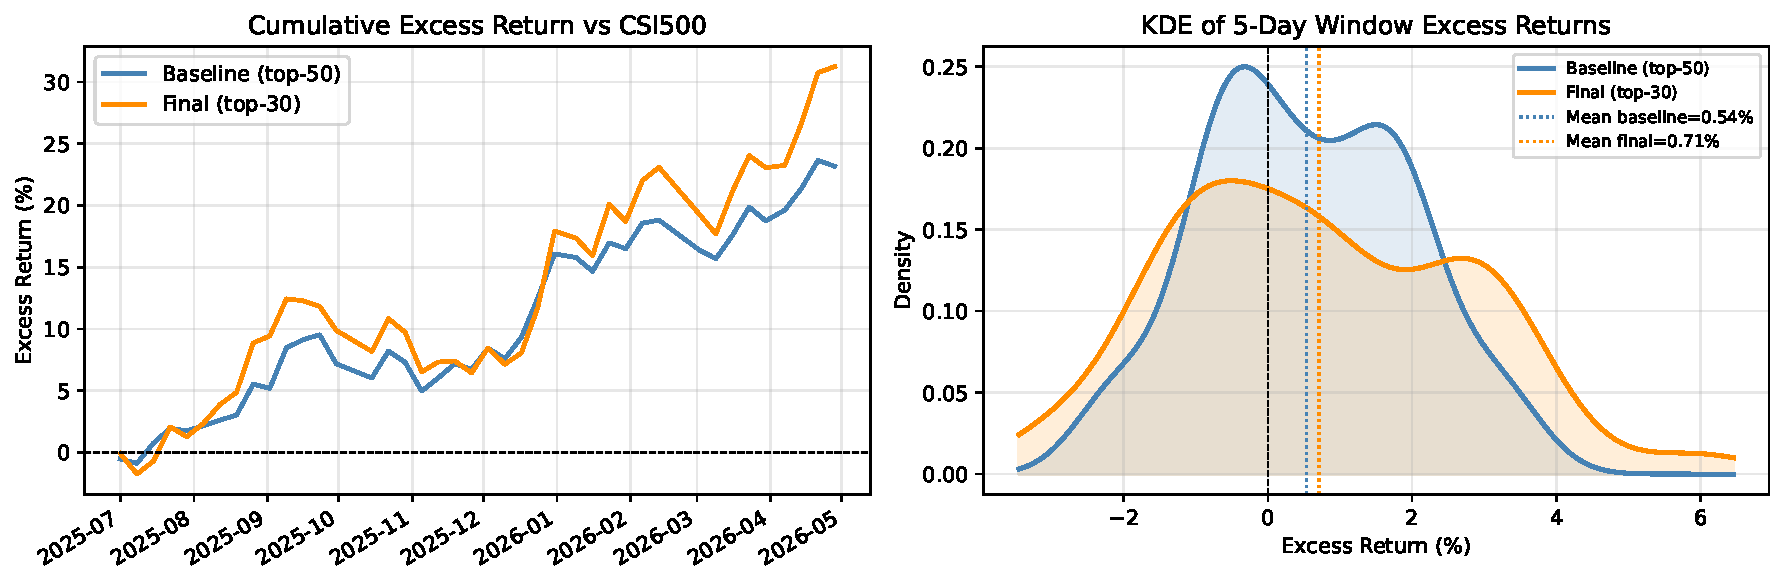
\includegraphics[width=\textwidth]{backtest_curves.pdf}
\caption{Left: Cumulative excess return over the CSI500 benchmark during the
test period (2025-07-01 to 2026-05-08). Right: Distribution of 5-day window
excess returns (KDE with mean marked).
Orange: LightGBM score-weighted top-30 (final model, $+42.84\%$ cumulative excess).
Blue: XGBoost baseline rank-weighted top-50 ($+23.18\%$).}
\end{figure}

%% ============================================================
\section{Analysis}\label{sec:analysis}
%% ============================================================

\subsection{What Worked}

\textbf{Industry neutralisation} was the single most impactful change,
improving test-set IC from $-0.009$ to $+0.026$. Without neutralisation,
the model learns to chase sector-rotation signals (e.g., all energy stocks
rising together), which have low persistence at weekly frequency. With
neutralisation, the model focuses on within-sector relative performance,
a more stable and predictable signal.

\textbf{Walk-forward retraining.} A static LightGBM model trained once on
the training set and applied throughout the test period underperforms the
walk-forward variant. Retraining every 20 days allows the model to adapt
to changing market conditions and prevents the degradation that occurs
when a fixed model is applied far outside its training distribution.

\textbf{A-share specific factors.} \texttt{amihud\_20d} is the
highest-importance feature (Table~\ref{tab:fimp}), consistent with the
illiquidity premium hypothesis in equity markets.
\texttt{overnight\_ratio\_20d} (rank 12) captures persistent informed
trading order flow, which is particularly informative in A-shares.

\textbf{Score-weighted portfolio construction.} Replacing linear rank
weighting with score weighting (proportional to shifted predicted magnitude)
improved test-set cumulative excess from $+31.25\%$ to $+42.84\%$ ($+11.6$pp).
The gain arises because the model's predicted return magnitudes are informative:
the top few stocks by predicted score are genuinely stronger signals, and
overweighting them relative to a flat rank weighting exploits this calibration.
The weighting scheme was selected on the validation set ($+66.55\%$ vs
$+51.90\%$ for rank-weighted, $n=27$ windows) and confirmed on the test set.

\subsection{What Did Not Work}

\textbf{Market-adjusted target} (subtracting index return from the label)
produced a portfolio with $-8.09\%$ cumulative excess. Beta carries genuine
information in A-shares: high-beta stocks systematically outperform during
bull phases. Removing the market component destroys this cross-sectional
signal.

\textbf{Exponential recency weighting} (half-life 126 days) performed worse
($+5.70\%$) than the unweighted 500d window. The exponential decay
over-discounts data from 2022--2023 bear market regimes, which contain
informative reversal and liquidity patterns that recur in later periods.

\textbf{LambdaRank objective.} Replacing the regression objective with
LambdaRank reduced performance. The likely failure mechanism is
information loss from discretisation: the 5-day forward return was binned
into 5 quantile labels (0--4) before training. This discards the
magnitude of returns within each bin --- a stock with $+8\%$ and one with
$+0.1\%$ both receive label 4, yet their true difference matters for
portfolio weighting.

\textbf{Multi-window ensemble} (250d + 500d models averaged). The two
models share 250 trading days of overlap in their training data and
produce correlated predictions. Averaging correlated outputs provides
negligible variance reduction while adding training cost; the walk-forward
backtest on the test set showed no improvement over the single 500d model.

\subsection{Limitations and Acknowledged Issues}

\textbf{LightGBM stochasticity.} \texttt{subsample} and
\texttt{colsample\_bytree} introduce randomness. Repeated runs with the
same configuration yield cumulative excess returns that vary by
$\pm 3$--$5$ percentage points. The reported numbers are from a single
run; true expected performance lies within this range around the reported
figures.

\subsection{Experiment Summary}

\begin{table}[h]
\centering
\begin{tabular}{p{7cm}p{7cm}}
\toprule
Experiment & Finding \\
\midrule
Industry neutralisation (SW Level-1)
  & IC: $-0.009 \to +0.026$; single most impactful change \\
Walk-forward retraining every 20 days
  & $+8$pp cumulative excess over static LightGBM \\
Market-adjusted target (raw $-$ index)
  & $-8.09\%$ cumulative excess; A-share beta is signal \\
Recency weighting (half-life 126d)
  & $+5.70\%$; discards informative historical regimes \\
XGBoost v2 (19 features)
  & $-0.30\%$; LightGBM-selected features add noise in XGBoost \\
LambdaRank objective (5-bin labels)
  & Underperformed regression baseline; return magnitude lost in discretisation \\
Multi-window ensemble (250d+500d)
  & No improvement; predictions too correlated \\
Top-30 vs top-40 vs top-50 (val set)
  & Top-30: $+50.45\%$, top-40: $+43.43\%$, top-50: $+37.63\%$; top-30 selected on val \\
Score-weighted vs rank-weighted (val set)
  & Score: $+66.55\%$, rank: $+51.90\%$, equal: $+38.69\%$; score-weighted selected on val \\
Final: LightGBM score-weighted top-30 (test set)
  & $+42.84\%$ cum.\ excess, win rate 59\%, IC IR $= 0.32$ \\
\bottomrule
\end{tabular}
\caption{Summary of all experiments.}
\end{table}

%% ============================================================
\section{Reproducibility}
%% ============================================================

\subsection{Pipeline}

\begin{verbatim}
# 1. Download data
python download_data.py --start 20220101 --end 20260430

# 2. Run self-test to reproduce reported IC metrics
python self_test.py

# 3. Generate submissions
python submit.py --as-of 20260430 --out submissions/submission1.csv
python download_data.py --update --end 20260508
python submit.py --as-of 20260508 --out submissions/submission2.csv

# 4. Validate
python validate_submission.py submissions/submission1.csv
python validate_submission.py submissions/submission2.csv
\end{verbatim}

Key packages: \texttt{xgboost}, \texttt{lightgbm}, \texttt{pandas},
\texttt{numpy}, \texttt{scipy}, \texttt{akshare}, \texttt{pyarrow}.
See \texttt{requirements.txt} for pinned versions.

\subsection{AI Assistance Acknowledgement}

LLMs (Claude) were used as a coding assistant for debugging, refactoring,
and drafting code. All model design decisions, feature engineering choices,
experimental directions, and result interpretations were produced by the
student. No LLM was used to directly generate portfolio weights or predict
stock returns. The baseline code originates from
\texttt{NYUSH-ML/ml-competition-sp26}.

\end{document}
